\section{实验}
\label{sec:experiment}
\begin{figure*}[!ht]
  \centering
  \begin{minipage}[b]{\linewidth} 	
  \subfloat[]{
    \begin{minipage}[b]{0.12\linewidth} 
      \centering
      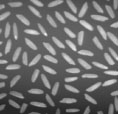
\includegraphics[width=\linewidth]{fig4_11}\vspace{1pt}
      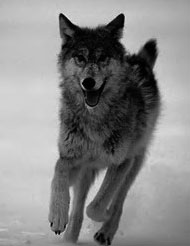
\includegraphics[width=\linewidth]{fig4_21}\vspace{1pt}
      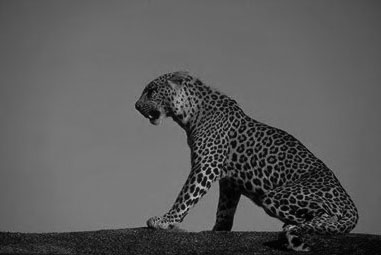
\includegraphics[width=\linewidth]{fig4_31}
       \end{minipage}
  }
    \subfloat[]{
    \begin{minipage}[b]{0.16\linewidth}
      \centering
      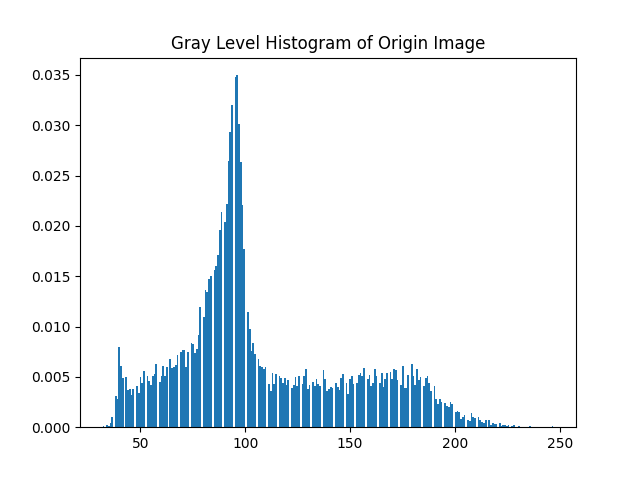
\includegraphics[width=\linewidth]{fig4_12}\vspace{2pt}
      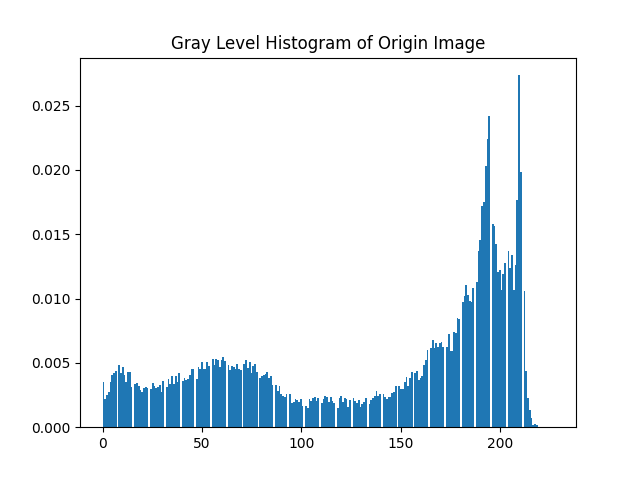
\includegraphics[width=\linewidth]{fig4_22}\vspace{2pt}
      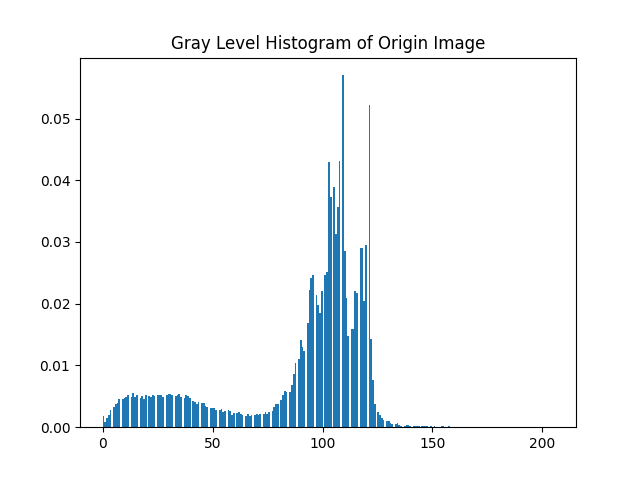
\includegraphics[width=\linewidth]{fig4_32}
     \end{minipage}
  }
   \subfloat[]{
    \begin{minipage}[b]{0.16\linewidth}
      \centering
       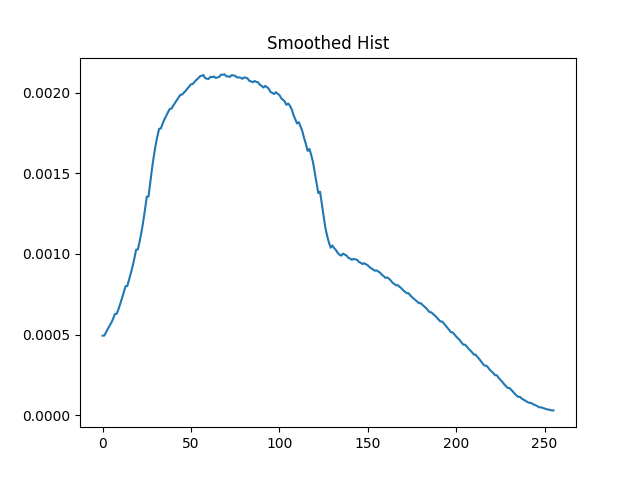
\includegraphics[width=\linewidth]{fig4_13}\vspace{2pt}
      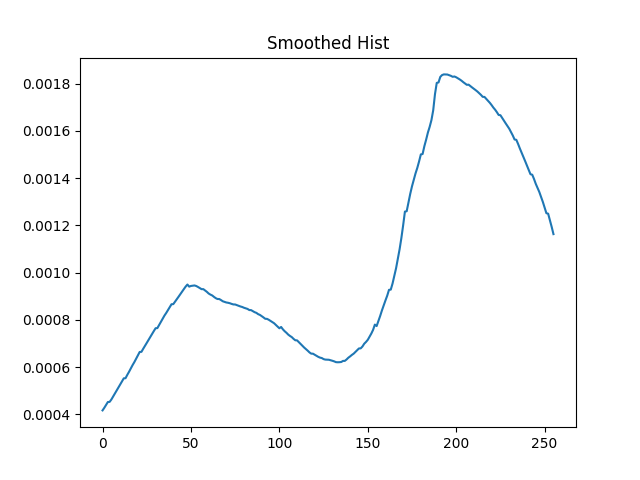
\includegraphics[width=\linewidth]{fig4_23}\vspace{2pt}
      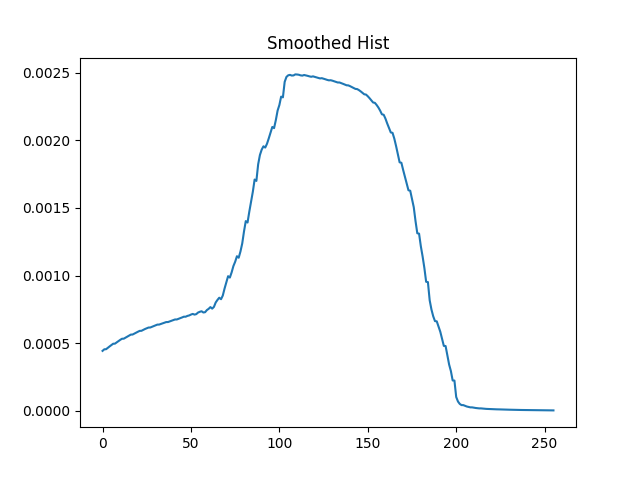
\includegraphics[width=\linewidth]{fig4_33}
       \end{minipage}
  }
  \subfloat[]{
    \begin{minipage}[b]{0.16\linewidth}
      \centering
       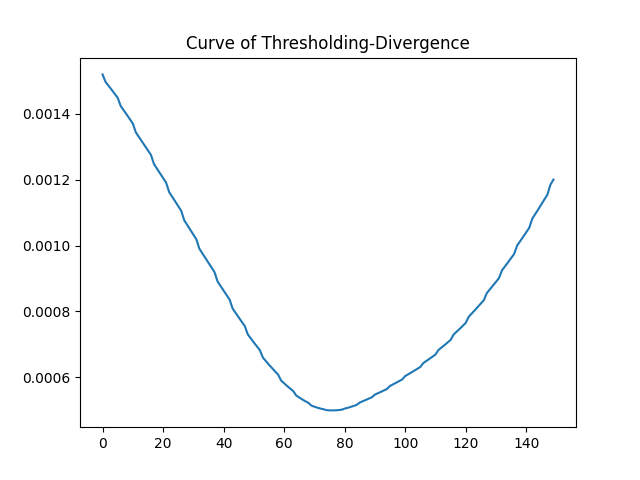
\includegraphics[width=\linewidth]{fig4_14}\vspace{2pt}
      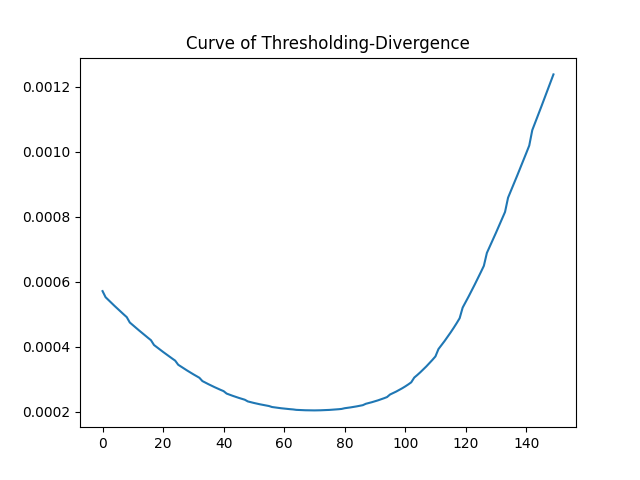
\includegraphics[width=\linewidth]{fig4_24}\vspace{2pt}
      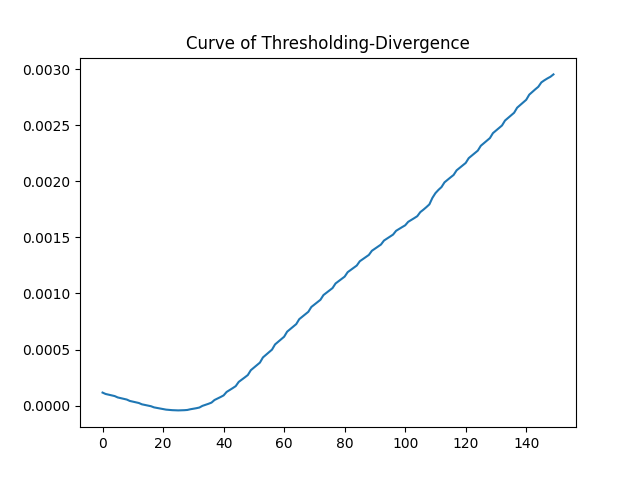
\includegraphics[width=\linewidth]{fig4_34}
       \end{minipage}
  }
   \subfloat[]{
    \begin{minipage}[b]{0.16\linewidth}
      \centering
       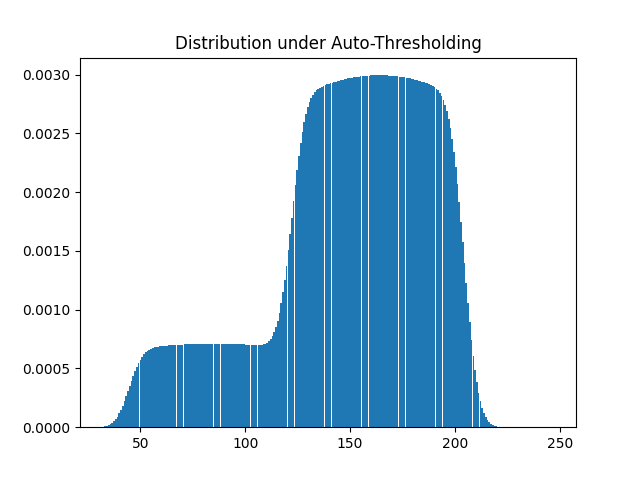
\includegraphics[width=\linewidth]{fig4_15}\vspace{2pt}
      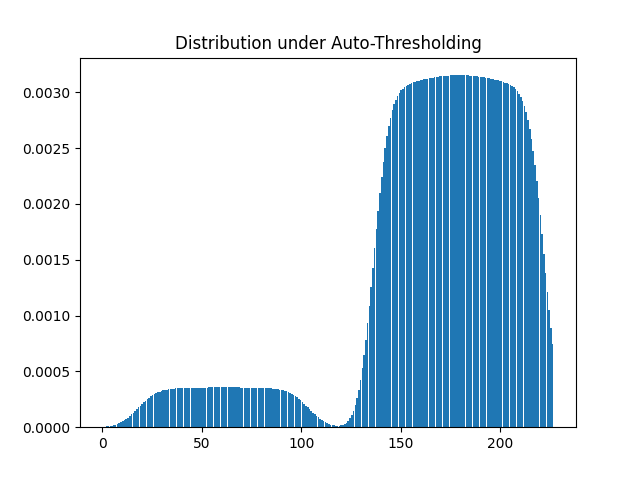
\includegraphics[width=\linewidth]{fig4_25}\vspace{2pt}
      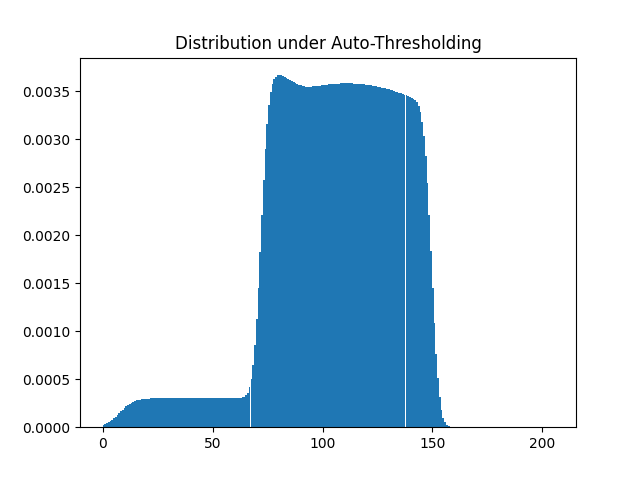
\includegraphics[width=\linewidth]{fig4_35}
       \end{minipage}
  }
  \subfloat[]{
    \begin{minipage}[b]{0.16\linewidth}
      \centering
       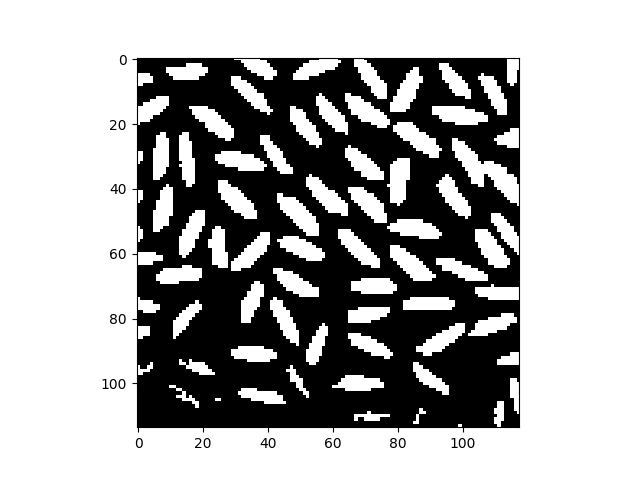
\includegraphics[width=\linewidth]{fig4_16}\vspace{2pt}
      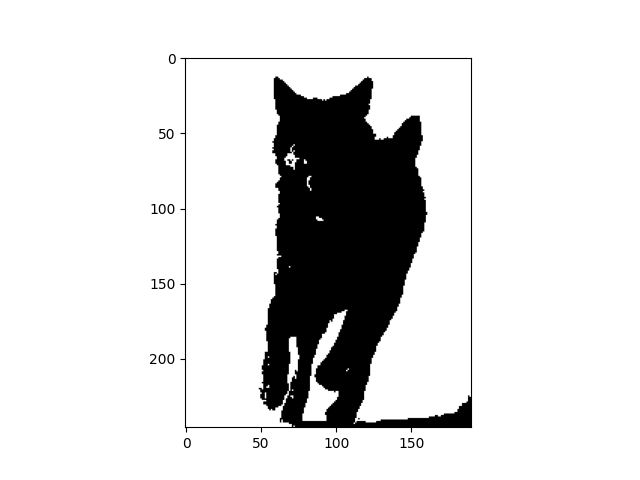
\includegraphics[width=\linewidth]{fig4_26}\vspace{2pt}
      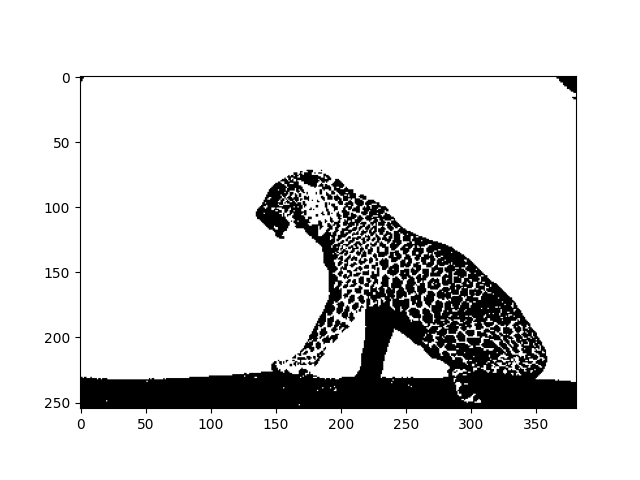
\includegraphics[width=\linewidth]{fig4_36}
       \end{minipage}
  }
  \end{minipage}
  \vfill
  \caption{基于直方图的自适应阈值分割结果:(a) 原始图像, (b) 灰度直方图, (c) 一维高斯滤波后的灰度信息图, (d) 阈值-散度曲线图, (e) 散度最小时拟合的灰度直方图, (f) 自适应阈值的分割结果.}
  \label{fig:auto_thresholding_result}
\end{figure*}

\subsection{基于人工设置阈值的分割结果}

设定三个不同阈值,分别为99、125和156,分割结果如图 \ref{fig:random_thresholding} 所示。可以看到对于同一幅图像来说,阈值设置过低时,背景中的噪声也会被划分到目标类别中,而当阈值设置过高时,目标中灰度值较低的部分被划入了背景部分。以 Test\_Img\_1 为例,在阈值为125时,分割效果较好,而在设置阈值为99时,分割结果中有部分背景噪声被分割到了目标中,而当阈值设置为156时,图像中的目标明显分割不全。此外,对于不同的图像而言,相同的阈值也会取得不同的分割效果。例如在阈值设置为125时, Test\_Img\_1 可以去的较好的分割效果,但 Test\_Img\_3 的分割结果质量很差。

\subsection{基于直方图的自适应阈值分割结果}

在一维高斯滤波滑动窗口大小为96,$\mu=0,\sigma=128$ 的自适应阈值分割结果如图 \ref{fig:auto_thresholding_result} 所示,得到的阈值如表 \ref{tab:thresholding} 所示:

\begin{table}[!ht]
\vspace{0.03cm}
\caption{基于直方图的自适应阈值分割方法阈值表}
\label{tab:thresholding}
\setlength{\tabcolsep}{4mm}{

\begin{tabular}{c|ccc}
\hline
 & Test\_Img\_1 & Test\_Img\_2 & Test\_Img\_3 \\
 \hline
阈值 & 126 & 120 & 75\\
\hline
\end{tabular}}
%\vspace{.4cm}
\end{table}

从图 \ref{fig:auto_thresholding_result} 可以看出,基于直方图的自适应阈值分割方法在三幅图像中均取得了较好的分割效果,尤其是对于 Test\_Img\_3 来说,该方法选取的阈值的分割结果远远好于人工设定的三个阈值的分割结果。而表  \ref{tab:thresholding} 则反映了由于不同图像的内容不同,其灰度值的分布也不相同,导致其阈值的选取变化也较大,基于直方图的自适应阈值分割方法可以根据不同图像的灰度值分布选取合适的分割阈值,从而可以大大减少人力工作。


但基于直方图的自适应阈值分割方法的性能还会受到一些参数选择的影响,例如滤波窗口大小的选择等,下面将对部分参数对分割结果的影响进行简单讨论。

\subsection{对比实验}

在本文实现的基于直方图的自适应阈值分割方法中,采用了一维高斯滤波器对图像的灰度直方图进行去噪,因此,除了滑动窗口大小的选择外,一维高斯滤波器的参数也对分割结果有一定的影响。这一部分,我们将对一维高斯滤波 $\sigma$ 大小和一维高斯滤波窗口大小对分割结果的影响进行讨论。

\subsubsection{一维高斯滤波 $\sigma$ 大小的影响}

在探究 $\sigma$ 大小对阈值选取和分割结果的影响时,固定其他参数不变,$\sigma$ 分别选取 16、128和256,在图像 Test\_Img\_2 上进行实验,阈值的选取如表 \ref{tab:sigma} 所示,分割结果如图 \ref{fig:sigma_result} 所示。

\begin{table}[!ht]
\vspace{0.03cm}
\caption{不同 $\sigma$ 一维高斯滤波得到的自适应阈值表}
\label{tab:sigma}
\setlength{\tabcolsep}{6.5mm}{

\begin{tabular}{c|ccc}
\hline
 & $\sigma=16$ & $\sigma=128$ & $\sigma=256$ \\
 \hline
阈值 & 145 & 120 & 114\\
\hline
\end{tabular}}
\end{table}

\begin{figure}[!ht]
	\vspace{-0.8cm}
  \centering
  \begin{minipage}[b]{\linewidth} 	
  \subfloat[]{
    \begin{minipage}[b]{0.3\linewidth} 
      \centering
      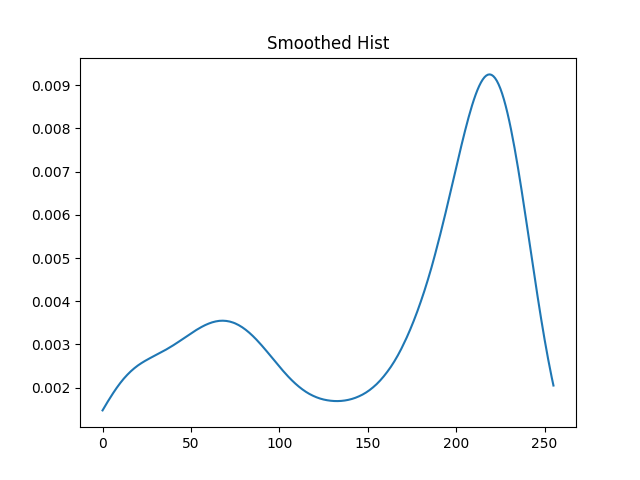
\includegraphics[width=\linewidth]{s_16_2}\vspace{1pt}
      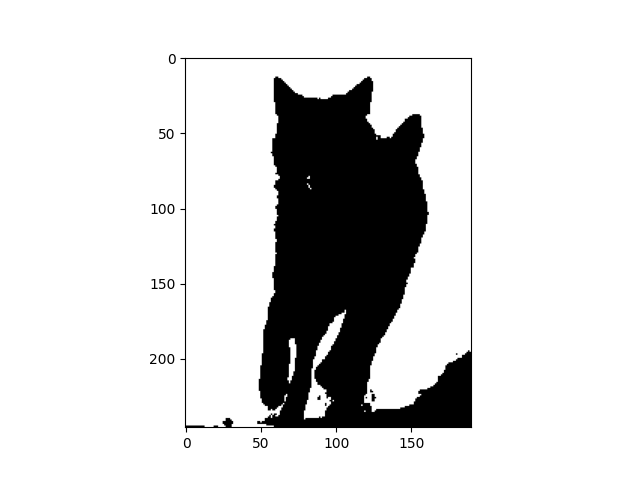
\includegraphics[width=\linewidth]{s_16_1}
       \end{minipage}
  }
    \subfloat[]{
    \begin{minipage}[b]{0.3\linewidth}
      \centering
      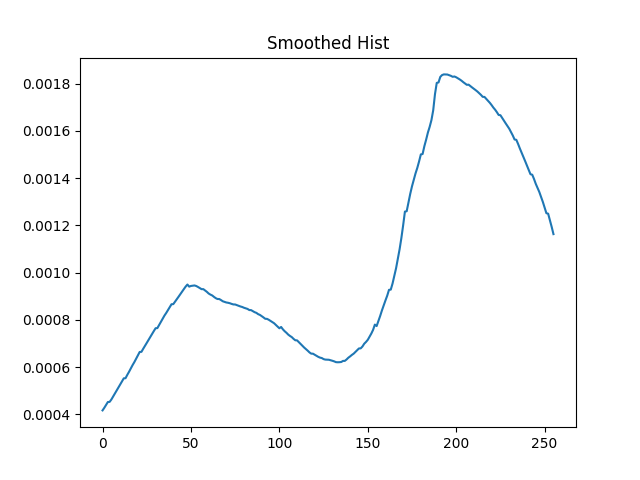
\includegraphics[width=\linewidth]{fig4_23}\vspace{2pt}
      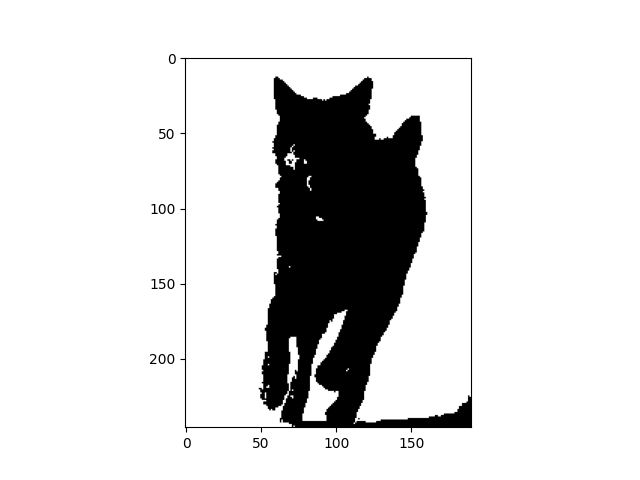
\includegraphics[width=\linewidth]{fig4_26}
     \end{minipage}
  }
   \subfloat[]{
    \begin{minipage}[b]{0.3\linewidth}
      \centering
       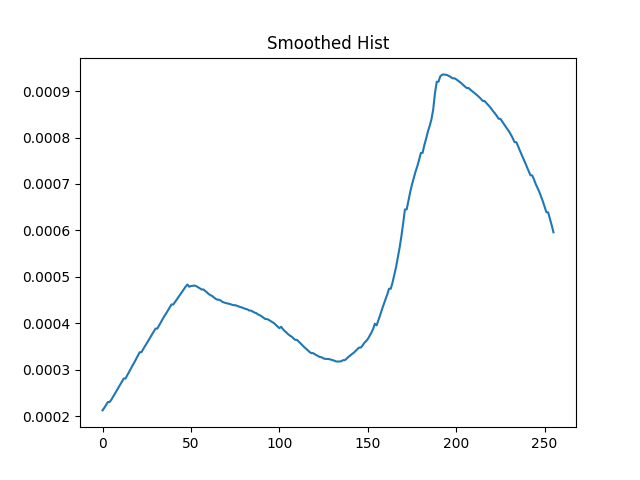
\includegraphics[width=\linewidth]{s_256_2}\vspace{2pt}
      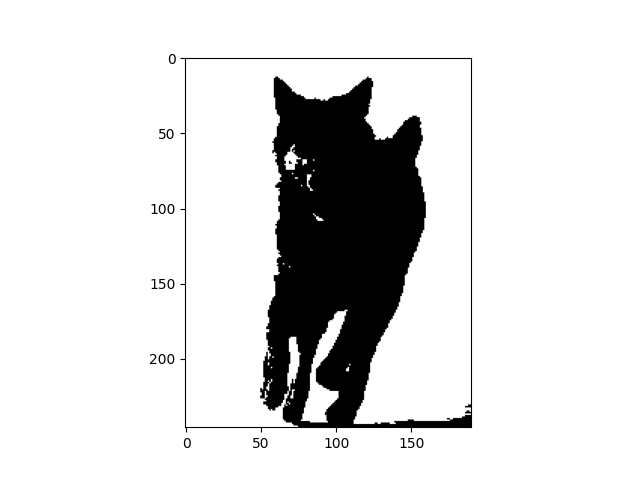
\includegraphics[width=\linewidth]{s_256_1}
       \end{minipage}
  }
  \end{minipage}
  \vfill
  \caption{不同 $\sigma$ 一维高斯滤波得到的自适应阈值分割结果:(a) $\sigma=16$, (b) $\sigma=128$, (c) $\sigma=256$.第一行为经过一维高斯滤波后的灰度分布统计图,第二行为基于自适应阈值分割的结果}
  \label{fig:sigma_result}
\end{figure}

结合表 \ref{tab:sigma} 和图 \ref{fig:sigma_result} 可以看出,随着 $\sigma$ 的增大,阈值的选取逐渐减小,对图片的分割结果也有比较大的影响。图像 Test\_Img\_2 中目标区域灰度值整体偏低,背景区域灰度值偏高,而随着阈值的增大,可以有效地减少背景中被错误分割到目标区域的像素数量(如图像右下部分的区域),但同时,目标中灰度值偏高的部分像素也会随之被分割到背景区域中(如狼的面部、脚等)。 

\subsubsection{一维高斯滤波窗口大小的影响}

在探究滤波滑动窗口大小对阈值选取和分割结果的影响时,固定其他参数不变,窗口大小分别选取 64、96和128,在图像 Test\_Img\_2 上进行实验,阈值的选取如表 \ref{tab:winsize} 所示,分割结果如图 \ref{fig:winsize_result} 所示。

\begin{table}[!ht]
\vspace{0.03cm}
\caption{不同滤波窗口大小得到的自适应阈值表}
\label{tab:winsize}
\setlength{\tabcolsep}{2.5mm}{

\begin{tabular}{c|ccc}
\hline
 & window size=64 & window size=96 & window size=128 \\
 \hline
阈值 & 160 & 120 & 112\\
\hline
\end{tabular}}
\end{table}

\begin{figure}[!ht]
	\vspace{-0.8cm}
  \centering
  \begin{minipage}[b]{\linewidth} 	
  \subfloat[]{
    \begin{minipage}[b]{0.3\linewidth} 
      \centering
      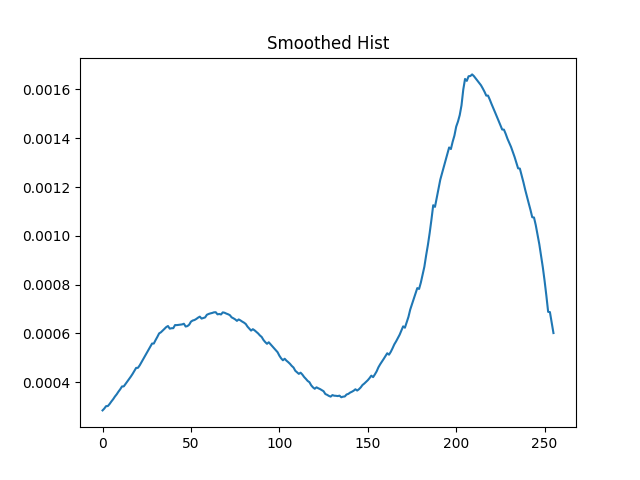
\includegraphics[width=\linewidth]{ws_64_1}\vspace{1pt}
      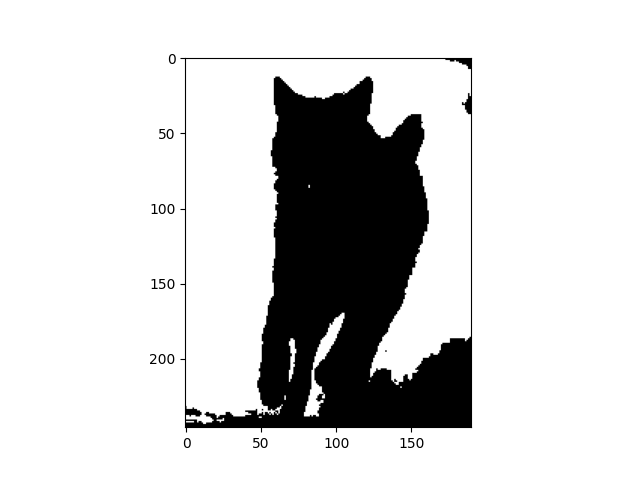
\includegraphics[width=\linewidth]{ws_64_2}
       \end{minipage}
  }
    \subfloat[]{
    \begin{minipage}[b]{0.3\linewidth}
      \centering
      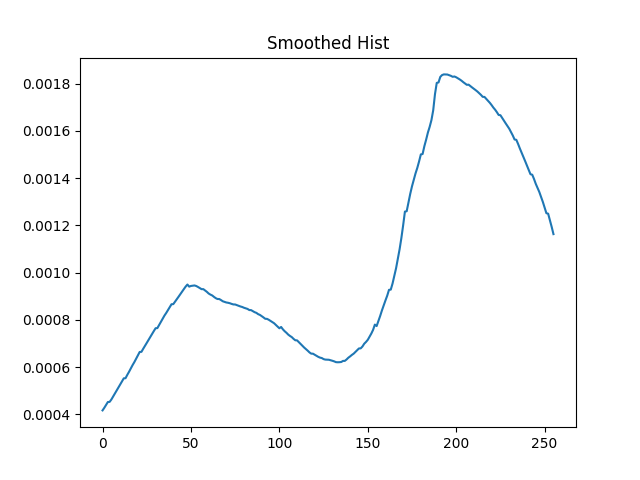
\includegraphics[width=\linewidth]{fig4_23}\vspace{2pt}
      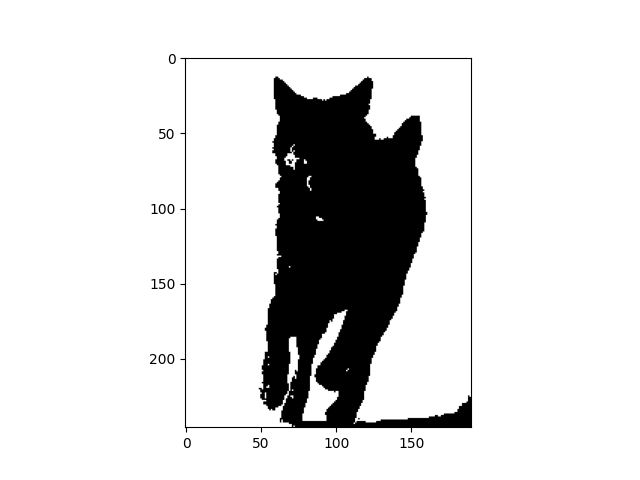
\includegraphics[width=\linewidth]{fig4_26}
     \end{minipage}
  }
   \subfloat[]{
    \begin{minipage}[b]{0.3\linewidth}
      \centering
       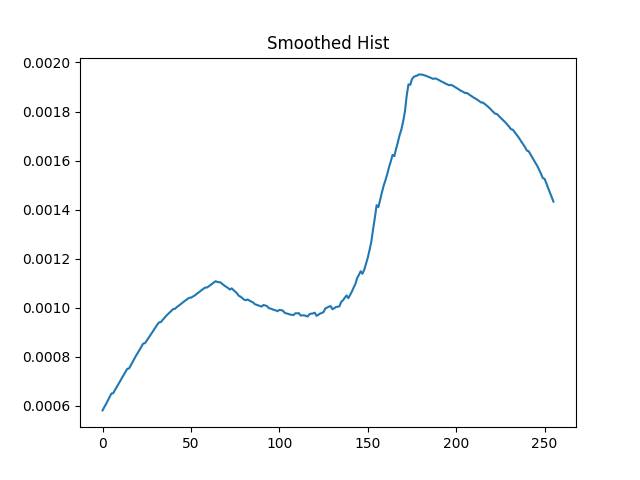
\includegraphics[width=\linewidth]{ws_128_1}\vspace{2pt}
      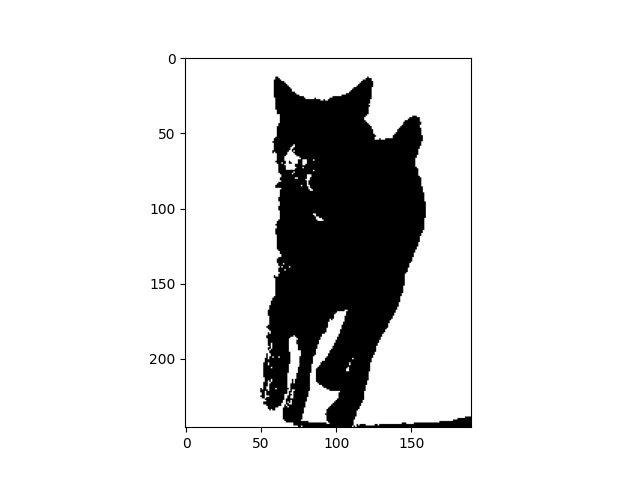
\includegraphics[width=\linewidth]{ws_128_2}
       \end{minipage}
  }
  \end{minipage}
  \vfill
  \caption{不同滤波窗口大小得到的自适应阈值分割结果:(a) window size=64, (b) window size=96, (c) window size=128.第一行为经过一维高斯滤波后的灰度分布统计图,第二行为基于自适应阈值分割的结果}
  \label{fig:winsize_result}
\end{figure}

结合表 \ref{tab:winsize} 和图 \ref{fig:winsize_result} 可以看出,随着滤波滑动窗口的增大,阈值的选取逐渐减小,对图片的分割结果也有比较大的影响。其对图片分割的影响在上一小节已经进行了阐述,此处不再赘述。滤波滑动窗口的增大会导致阈值的选取减小,是由于滑动窗口增大在总体趋势上会导致灰度值分布更加平滑,噪声更少,使得对混合高斯分布的拟合更加准确。

综合上述实验结果来看,基于直方图的自适应阈值分割方法相比较人工设定阈值更加高效、准确,但其阈值的选取也受到其他因素的影响,如滤波滑动窗口的大小等。同时,也不难分析得出该方法对噪声敏感,鲁棒性较差。
